\chapter{Implementace příkazů}

V této kapitole popisuji analýzu a realizaci linuxových příkazů, které jsou v simulátoru implementovány. Příkazy jsou nejrozsáhlejší částí mojí práce na simulátoru, protože jsem u každého příkazu nejprve musel složitě zjišťovat, jak funguje a jak se chová v případě zadání nestandardních parametrů. Parsování příkazů bylo prací pořád stejnou a nezábavnou. 

Nejprve popisuji zpracování příkazové řádky, pak obecné principy pro zpracování všech příkazů a nakonec popisuji analýzu a implementaci konkrétních příkazů.



%------------------------------------------------------------------------------------------------------

\section{Popis zpracování příkazové řádky}

Příkazovou řádku virtuálního počítače obsluhuje třída \verb|Konsole| (více v \ref{impl_komunikacni_vrstva}), jež načítá textová data posílaná uživatelem až do sekvence \verb|\r\n|, kdy načítání zastaví a načtený řádek předá svému parseru. Každá \verb|Konsole| má svůj vlastní parser příkazů, který zpracovává jen jí poslané řádky a na ně odpovídá. \verb|Konsole| zavolá jeho metodu \verb|zpracujRadek|, která separuje jednotlivá slova řádku a pak podle prvního slova, které by mělo být názvem příkazu, spustí odpovídající příkaz. Příkazům \verb|Konsole| poskytuje metody \verb|posliRadek| a \verb|posli|, pomocí kterých příkazy vypisují svůj výstup uživateli do konzole.

Architektura tříd pro zpracování příkazové řádky je celkem složitá, jak je vidět na obrázku \ref{obr_prikazy}. Všechny třídy mají jednoho předka, kterého jsme pojmenovali \verb|Abstraktni|. Každý příkaz má svoji vlastní třídu, již \verb|ParserPrikazu| vytvoří pro každé použití příkazu nově, jde tedy o použití návrhového vzoru singleton. V následujících odstavcích popisuji funkce jednotlivých tříd.

% třídy pro zpracování příkazů
\begin{figure}[h]
\begin{center}
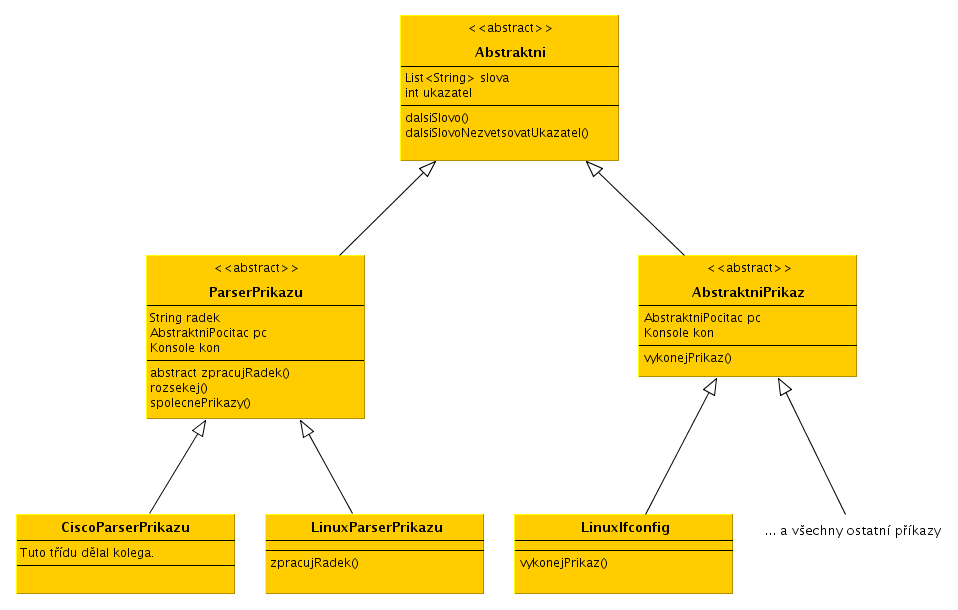
\includegraphics[width=14cm]{obrazky/prikazy}
\caption{Třídy pro zpracování příkazové řádky}
\label{obr_prikazy}
\end{center}
\end{figure}


\subsection{Třída Abstraktni}

Tato třída je abstraktním předkem všech ostatních tříd sloužících ke zpracování příkazů. Obsahuje pro parsování velmi důležitou metodu \verb|dalsiSlovo| a seznam slov jednoho řádku. Tato metoda postupně vrací jednotlivá slova ze seznamu. Je využívána skoro všemi potomky třídy \verb|Abstraktni| k parsování řádky. Dále jsou v této třídě různé statické metody využívané jednotlivými příkazy, například metoda \verb|zarovnej| pro zarovnání slova v řetězci, metoda \verb|cekej|, která čeká zadaný počet milisekund a jiné.

\subsection{Třída ParserPrikazu}

Instanci jednoho z potomků této třídy, tedy \verb|LinuxParsePrikazu| nebo \verb|CiscoParserPrikazu|, si vytváří při své inicializaci třída \verb|Konsole|, které slouží ke zpracování příkazové řádky. Jeho hlavní metodou je abstraktní \verb|zpracujRadek|, která je implementována v jeho potomcích a zpracovává jeden řádek, který uživatel do konzole napsal. K tomu používá metodu \verb|rozsekej|, jejímž autorem je můj kolega, která řádek zadaný jako \verb|String| \uv{rozseká} na jednotlivá slova a to tak, že jako oddělovače bere bílé znaky, tj. mezery a tabulátory. Rozsekaná slova pak uloží do seznamu řetězců \verb|slova|, který zdědila od svého předka třídy \verb|Abstraktni|. Třída \verb|LinuxParsePrikazu| podle prvního slova, které by mělo být názvem příkazu, vyvolá konstruktor třídy odpovídajícího příkazu. Nejdříve kontroluje, jestli příkaz není společným příkazem pro linuxový i ciscový počítač (příkaz \verb|uloz| nebo \verb|save|) a poté se snaží najít odpovídající linuxový příkaz. Jestliže uživatelem zadaný příkaz neexistuje nebo není implementován, vypíše \verb|LinuxParsePrikazu| uživateli řetězec \verb|bash: command not found| a zpracování řádku ukončí.


\subsection{Třída AbstraktniPrikaz}

Tato třída je potomkem třídy \verb|Abstraktni| a předkem tříd všech příkazů. Nemá žádnou důležitou metodu, ale parametry \verb|abstraktniPocitac pc| a \verb|konsole kon|, což jsou odkazy na počítač, na kterém příkaz probíhá a na konzoli, která ho vyvolala.



%------------------------------------------------------------------------------------------------------

\section{Společné znaky příkazů}

Příkazy, které jsem implementoval mají mnoho společného. Všechny jsou potomkem třídy \verb|AbstraktniPrikaz|, který je potomkem třídy \verb|Abstraktni|. Text, který byl uživatelem zadán, mají uložen v seznamu řetězců \verb|slova|. V konstruktoru příkazu je postupně voláno několik privátních metod. Metodou \verb|zparsujPrikaz| se nejprve parsuje vstup, většinou pomocí metody \verb|dalsiSlovo| zděděné ze třídy \verb|Abstraktni|. Při parsování se nastavují různé parametry příkazu, které uživatel zadal. Metoda \verb|zkontrolujPrikaz| kontroluje, jestli jsou nastaveny správné parametry, a jestli byly zadány všechny. Potom metoda \verb|vykonejPrikaz| příkaz vykoná, to znamená, že změní konfiguraci počítače například u příkazu \verb|ifconfig|, nebo že provede nějakou jinou akci, například u příkazu \verb|ping| pošle několik paketů. Během těchto tří metod jsou ukládány případné chyby zadaného příkazu. Úplně nakonec příkaz vypíše případné chybové hlášení. Tento postup byl zvolen proto, že sladit správné pořadí vypisovaných chybových hlášení s postupem kontroly jednotlivých parametrů by bylo velmi náročné a nepřehledné. Příkazy svůj výstup posílají pomocí metod \verb|posli| a \verb|posliRadek| třídy \verb|Konsole|.



%------------------------------------------------------------------------------------------------------

\section{Příkaz ifconfig}


\subsection{Teoretický úvod}

\verb|ifconfig| (zkratka \textbf{i}nter\textbf{f}ace \textbf{config}urator) \uv{je utilita unixových systémů, která slouží ke konfiguraci, kontrole  a vypsání informací o parametrech síťových rozhraní z příkazové řádky.}\cite{wiki_ifconfig}. Pomocí této utility lze například vypsat parametry síťových rozhraní, nastavit IP nebo mac adresy, nastavit masky nebo \uv{nahodit} nebo \uv{shodit} rozhraní. Kromě toho, že \verb|ifconfig| nastavuje rozhraní, přidává nebo maže i záznamy v routovací tabulce, je-li to potřeba.


\subsection{Rozsah implementace v simulátoru}

V simulátoru musí \verb|ifconfig| umět nastavovat a mazat adresy IP a nastavovat masky. Samozřejmě také musí vypisovat nastavené parametry rozhraní. Změna mac adresy naproti tomu v našem simulátoru není vůbec potřeba. Parser příkazu \verb|ifconfig| je ale implementován i pro parametry \verb|add|, \verb|del|, \verb|up| a \verb|down|.

Zde uvádím příklady užití ifconfigu, které simulátor podporuje:
\begin{verbatim}
ifconfig eth0                             vypíše parametry rozhraní eth0
ifconfig eth0 192.168.1.1                 nastaví adresu na rozhraní eth0
ifconfig eth0 10.0.0.1/8                  nastaví adresu s maskou
ifconfig eth0 10.0.0.2 netmask 192.0.0.0  nastaví adresu s maskou
\end{verbatim}


\subsection{Analýza ifconfigu na skutečném počítači}\label{ifconfig_analysa}

Oproti jiným příkazům má \verb|ifconfig| pro simulaci jednu obrovskou nevýhodu: chybný parametr nezpůsobí ukončení příkazu, ale příkaz se dále provádí. Některé parametry je možné zadat vícekrát. Zjišťovat, jak se \verb|ifconfig| chová, proto bylo mnohem náročnější, než u ostatních příkazů. Zde popisuji výsledky této práce.

IP adresu je možné příkazu zadat vícekrát, všechno, co nelze zparsovat jinak se považuje za IP adresu. Je-li zadáno více adres, použije se adresa, které předchází první špatné adrese. Například příkazem:
\begin{verbatim}
ifconfig eth0 1.1.1.1 2.2.2.2 3.3.3.3
\end{verbatim}
se nastaví poslední adresa, tj. \verb|3.3.3.3|. Příkazem
\begin{verbatim}
ifconfig eth0 1.1.1.1 blablabla 3.3.3.3
blablabla: unknown host
ifconfig: `--help' vypíše návod k použití.
\end{verbatim}
nastaví se adresa před první špatnou adresou, tj. \verb|1.1.1.1|. Adresu je možné zadat i s délkou prefixu za lomítkem. Je-li zadáno více adres a u jedné z nich je zadána délka prefixu, nastaví se taková maska, i když se tato adresa nepoužije. Například
\begin{verbatim}ifconfig eth0 1.1.1.1/1 2.2.2.2/2 3.3.3.3\end{verbatim}
nastaví adresu 3.3.3.3 s maskou 192.0.0.0, použije se tedy délka prefixu zadaná u druhé adresy. Adresa na rozhraní se maže nastavením adresy na 0.0.0.0.

Maska se nastavuje buď zadáním délky prefixu, jak je popsáno výše, nebo parametrem netmask. Zadá-li uživatel masku oběma způsoby, má přednost délka prefixu před parametrem netmask. Například
\begin{verbatim}ifconfig eth0 2.2.2.2/2 netmask 255.255.0.0\end{verbatim}
nastaví masku 192.0.0.0. Při změně IP adresy se automaticky mění i maska a to tak, že se maska dopočítá podle třídy IP adresy. Je-li tedy nejprve zadána maska parametrem netmask a teprve potom IP adresa, parametr netmask nemá žádnou účinnost. Například
\begin{verbatim}ifconfig eth0 netmask 255.255.255.0 1.1.1.1\end{verbatim}
nastaví adresu 1.1.1.1 s maskou 255.0.0.0.0, protože adresa 1.1.1.1 je třídy \verb|A|.

Příkaz \verb|ifconfig| promítá změny i do routovací tabulky. Změní-li se adresa na rozhraní, všechny záznamy na toto rozhraní se z tabulky vymažou. Při nastavení IP adresy se do routovací tabulky přidá záznam typu \verb|U| pro síť, ze které je tato adresa. Například při nastavení adresy
\begin{verbatim}ifconfig eth0 192.168.1.1/24\end{verbatim}
se do routovací tabulky přidá tento záznam:
\begin{verbatim}
Adresát         Brána           Maska           Přízn Metrik  Rozhraní
192.168.1.0     0.0.0.0         255.255.255.0   U     0       eth0
\end{verbatim}

Při zadání chybného vstupu se vykoná jen správná část příkazu a o těch špatných se vypíší chybová hlášení. Ty jsou vypisována v tomto pořadí:
\begin{enumerate}
\item špatný přepínač - příkaz se neprovádí
\item špatná adresa - žádná další chybová hlášení se nevypisují
\item špatné rozhraní
\item zakázaná adresa
\item špatné adresy parametrů \verb|add| nebo \verb|del|
\item chyba v gramatice
\end{enumerate}

Ostatními parametry se v tomto odstavci nezabývám, protože v simulátoru nejsou podporovány.


\subsection{Implementace v simulátoru}

V konstruktoru třídy \verb|LinuxIfconfig| jsou popoředě volány tyto metody: \verb|parsujPrikaz|, \verb|zkontrolujPrikaz|, \verb|vypisChybovyHlaseni| a \verb|vykonejPrikaz|. Parsování se v tomto příkaze neprovádí s využitím metody \verb|dalsiSlovo|, což by bylo dobré ještě upravit. Na rozdíl od skutečného ifconfigu se parsuje celý řádek, skutečný ifconfig parsování zastaví, když dojde ke špatnému přepínači nebo ke špatné adrese. Při parsování se parametry ukládají jako řetězce a ty jsou kontrolovány metodou \verb|zkontrolujPrikaz|. V tomto příkazu jsou chybová hlášení vypisována již před samotným provedením příkazu a to v pořadí uvedeném v předchozím odstavci. Příkaz \verb|ifconfig| se metodou \verb|vykonejPrikaz| nakonec provede tak, aby to co nejvíce odpovídalo pravidlům uvedným v \ref{ifconfig_analysa}. Parametry \verb|add| a \verb|del| jsou v parsetu a kontrole implementovány, ale metoda \verb|vykonejPrikaz| je zatím ignoruje.


\subsection{Možnosti dalšího vylepšení}

Tento příkaz jsem implementoval jako první, kdy jsem s implementací příkazů ještě neměl zkušenosti, proto by se dal ještě v některých věcech vylepšit. Bylo by dobré přepsat metodu \verb|parsujPrikaz| tak, aby využívala metodu \verb|dalsiSlovo|, čímž by se zjednodušila, a dále ji předělat tak, aby se po špatné adrese již dále nic neparsovalo. Bylo by též dobré implementovat i parametry \verb|up| a \verb|down|, s jejichž podporou se v analýze nepočítalo.


\subsection{Známé odchylky}

Zde uvádím známé odchylky implementace v simulátoru od skutečného příkazu na reálném počítači.\\
\verb|ifconfig eth0 netmask 255.0.0.0 2.2.2.2/2| ve skutečnosti spadne kvůli prefixu za adresou, v simulátoru to ale projde.\\
\verb|ifconfig eth0 blabla netmask 255.255.255.0| ve skutečnosti žádnou masku nenastaví, protože přestane parsovat už u blabla.\\
\verb|ifconfig eth0 netmask 255.255.255.0 10.0.0.1| by měl nastavit masku na 255.0.0.0, v simulátoru se nastaví 255.255.255.0



%------------------------------------------------------------------------------------------------------

\section{Příkaz route}

Příkaz route je utilita, která umožňuje administrátorovi vypisovat a měnit záznamy v routovací tabulce. Uvedu zde pár praktických příkladů:
\begin{verbatim}
route                                       # vypíše routovací tabulku
Směrovací tabulka v jádru pro IP
Adresát         Brána           Maska           Přízn Metrik Rozhraní
192.168.1.0     0.0.0.0         255.255.255.0   U     0      eth0
0.0.0.0         192.168.1.2     0.0.0.0         UG    0      eth0

route add -net 10.0.0.0/8 gw 192.168.1.3    # Přidá záznam typu UG pro
   # síť 10.0.0.0/8 na bránu 192.168.1.3
route del -net 10.0.0.0/8                   # Odebere minule přidaný záznam
\end{verbatim}


\subsection{Analýza příkazu route na skutečném počítači}

Oproti příkazu \verb|ifconfig| má příkaz \verb|route| jasně definovanou gramatiku a při jakékoliv chybě v příkazu se příkaz neprovádí, proto byla implementace tohoto příkazu podstatně jednoduší. Příkaz má 2 hlavní akce, \verb|add| na přidávání záznamů a \verb|del| na jejich mazání. Nápověda uvádí ještě akci \verb|flush|, která ale není běžně podporována. Obě známé akce mají stejnou gramatiku. Parametr \verb|-net| přidá nebo odebere záznam pro síť, parametr \verb|-host| pro jednu adresu, tzn. záznam s maskou 255.255.255.255. Parametr \verb|gw| slouží k nastavení brány přidávanému nebo odebíranému záznamu, parametr \verb|dev| k nastavení rozhraní a parametr \verb|netmask| k nastavení masky přidávanému nebo odebíranému záznamu. Maska může být stejně jako v příkazu \verb|ifconfig| zadána parametrem \verb|netmask| nebo pomocí délky prefixu za lomítkem, např. \verb|10.0.0.0/16|. Při použití parametru \verb|-net| musí být vždy maska nějakým způsobem zadána. Adresát, tzn. parametr \verb|-net| nebo \verb|-host| musí být vždy prvním parametrem akce, na pořadí dalších parametrů již nezáleží. Parametry \verb|-host| a \verb|dev| není nutno psát. Žádný parametr nemůže být zadán vícektrát. Akce \verb|add| vyžaduje aspoň jeden z parametrů \verb|gw| nebo \verb|dev|. Narazí-li se při provádění přikazu na chybu, je vypsáno chybové hlášení a příkaz se ukončí, aniž by se vykonala jeho správná část.


\subsection{Implementace v simulátoru}

Implementoval jsem parametry \verb|-host|, \verb|-net|, \verb|netmask|, \verb|dev| a \verb|gw|. Parser tohoto příkazu je psán za pomocí metody \verb|dalsiSlovo| celkem přehledně, každý parametr se parsuje vlastní metodou. Parser též kontroluje správnost příkazu, vypisuje chybová hlášení a nastavuje parametry. Metoda \verb|vykonejPrikaz| upravuje nebo vypisuje routovací tabulku příslušného počítače.


\subsection{Odchylky}

Akce \verb|flush| sice není na normální počítači implementována, avšak v simulátoru jsem ji implementoval s tím, že simulátor vypíše varovné hlášení:
\begin{verbatim}
linux1:~# route flush
psi simulator: Flush normalne neni podporovano, ale routa se v simulatoru
smazala.
Spravny prikaz je: "ip route flush all"
\end{verbatim}



%------------------------------------------------------------------------------------------------------

\section{Příkaz ping}

Tento příkaz posílá ICMP pakety typu \verb|request| (žádost o odpověď) a přijímá pakety typu \verb|ICMP reply|. Uživateli umožňuje prověřit funkčnost spojení mezi dvěma počítači v síti.


\subsection{Analýza skutečného pingu}

Příkazu musí uživatel zadat cílovou adresu, na kterou se chce \uv{dopingnout}. Dále je možné použít několik přepínačů. Přepínačem \verb|-c| si uživatel určí, kolik paketů chce poslat, není-li tento parametr zadán, posílaji se pakety pořád, dokud uživatel příkaz nezastaví \verb|Ctrl+C|. Parametrem \verb|-s| je možné specifikovat velikost posílaného paketu, parametrem \verb|-i| se specifikuje interval mezi odesláním dvou paketů. Parametrem \verb|-t| je možné zadat \verb|ttl| odchozích paketů. Parametr \verb|-b| umožňuje posílat \verb|icmp request| na broadcastovou adresu a parametr \verb|-q| potlačuje výstup příkazu. Parametr \verb|-b| není v simulátoru podporován. Například příkaz:
\begin{verbatim}
ping -c10 -i 0.1 -s1000 -t 23  192.168.2.2
\end{verbatim}
pošle 10 paketů v intervalu 0,1 sekundy o velikosti 1000 bytů s ttl 23 na adresu 192.168.2.2. Na pořadí parametrů nezáleží, jejich hodnoty můžou být uvedeny bez mezery i s ní. U tohoto příkazu lze zadat přepínače i po IP adrese.


\subsection{Implementace v simulátoru}

Virtuální pakety, které si předávají virtuální počítače našeho simulátoru, si nesou i odkaz na příkaz, který je vyvolal. To proto, aby když počítači dorazí \verb|icmp reply| počítač věděl, který příkaz je původcem tohoto paketu. Proto všechny příkazy, které v našem simulátoru posílají pakety jsou potomkem abstraktní třídy \verb|AbstraktniPing|, jejíž abstraktní metodu \verb|zpracujPaket| volá přímo metoda počítače, který paket přijala. Tato třída má také metodu \verb|aktualizujStatistiky|, která spočítá konečné statistiky příkazu.

Parser tohoto příkazu je podobný jako v ostatních příkazech, pomocí metody \verb|dalsiSlovo| se parsují jednotlivé parametry. Příkaz nemá zvláštní metodu pro kontrolu pro výpis chybových hlášení. Metoda \verb|vykonejPrikaz| posílá pomocí metody \verb|posliIcmpRequest| třídy \verb|AbstraktniPocitac| jednotlivé pakety a pak je metodou \verb|zpracujPaket| zpracovává.

Čas odezvy vypisovaný tímto příkazem není skutečný, ale každý počítač procházejícímu paketu do parametru čas přičte náhodně vygenerovanou hodnotu a to tak, aby hodnoty byly přibližně stejné, jako jsou v laboratořích předmětu PSI.


\subsection{Odchylky v implementaci}

Protože program telnet, přes který se budou uživatelé simulátoru přihlašovat k počítačům neumí přeposílat \verb|Ctrl+C|, musím v našem simulátoru mít nastavený výchozí počet odesílaných paketů na 4, aby uživatel tento příkaz mohl nějak zastavit. Toto je velký rozdíl oproti skutečnému pingu na linuxu, ale neměl jsem jinou možnost.

Parametr \verb|-i|, kterým se nastavuje interval mezi odesláním dvou paketů, se musí v simulátoru zadat tak, aby mezi \verb|-i| a hodnoutou byla mezera. Není tedy možné napsat \verb|-i0.5|.

V simulátoru musí být oproti skutečnosti přepínače napsané před adresou. Ve skutečnosti to není nutné. Tento nedostatek ještě opravím.



%------------------------------------------------------------------------------------------------------

\section{Příkaz traceroute}

Program traceroute slouží k analýze počítačové sítě. Vypisuje uzly (resp. směrovače) na cestě datagramů od zdroje až k zadanému cíli. Uzly jsou zjišťovány pomocí snížení hodnoty TTL v hlavičce datagramů.\cite{wiki:traceroute}.


\subsection{Popis činnosti}

Příkaz posílá pakety ICMP request na cílovou adresu, kterým postupně zvyšuje \verb|ttl|, dokud nedojte od cílového počítače paket ICMP reply. Počítače, které paket nemohou dále poslat, protože mu \verb|ttl| vypršelo, posílají zdrojovému počítači zprávu ICMP time exceeded. Podle těchto zpráv příkaz zjistí, kterými uzly procházejí pakety k cílové adrese.

Příklad výpisu příkazu:
\begin{verbatim}
neiss: ~/smazat$ traceroute -n 89.190.94.58
traceroute to 89.190.94.58 (89.190.94.58), 30 hops max, 60 byte packets
 1  192.168.1.20  0.833 ms  1.257 ms  1.691 ms
 2  10.4.71.1  66.723 ms  67.245 ms  69.029 ms
 3  89.190.94.2  69.648 ms  70.088 ms  70.422 ms
 4  89.190.94.58  70.893 ms  71.261 ms  74.190 ms
\end{verbatim}


\subsection{Implementace}

Třída příkazu \verb|traceroute| dědí ze třídy \verb|AbstraktniPing|, aby odkaz na ní mohl být posílán spolu s paketem. Příkaz nemá prakticky žádný parser, jediná povolená syntaxe tohoto příkazu je \verb|traceroute <adresa>|. Pokud uživatel zadá neodpovídající vstup, vypíše se mu hlášení, jaká je jediná povolená syntaxe. Příkaz funguje na stejném principu jako příkaz skutečný, jak je popsáno v předchozím odstavci.



%------------------------------------------------------------------------------------------------------

\section{Příkaz exit}

Příkaz \verb|exit| je jedinou korektní možností ukončení relace. Zavolá metodu \verb|ukonciSpojeni| třídy \verb|Konsole|, čímž ukončí běh její metody \verb|run| a tak se spojení ukončí.



%------------------------------------------------------------------------------------------------------

\section{Příkaz ip}

Příkaz \verb|ip| je plnohodnotnou náhradou za příkazy \verb|ifconfig|, \verb|route|, \verb|arp|. Umožňuje však i pokročilejší správu síťových nastavení\cite{prikaz_ip}. Já jsem z tohoto příkazu ve svém simulátoru implementoval jeho dva základní podpříkazy \verb|addr| pro nastavení parametrů rozhraní a \verb|route| pro manipulaci se směrovací tabulkou.


\subsection{Implementace}

Příkaz \verb|ip| je implementován třídou \verb|LinuxIp|. Jeho podpříkazy \verb|addr| a \verb|route| ale byly implementovány samostatně, to znamená, že jsem pro každý podpříkaz vytvořil vlastní třídu. Třída \verb|LinuxIp| parsuje přepínače a jméno podpříkazu. Je-li napsaný podpříkaz podporován, spustí odpovídající třídu, která pak funguje stejně jako samostatný příkaz. Není-li podporován, vypíše o tom hlášení.

Parsování příkazu \verb|ip| má jednu zvláštnost. Není totiž nutné, aby uživatel psal všechny terminály, ale místo některých lze napsat třeba jen první písmeno, které terminál jednoznačně určuje. Tak například místo řádku
\begin{verbatim}
ip addr add 1.1.1.1 dev eth0
\end{verbatim}
lze jednoduše napsat
\begin{verbatim}
ip a a 1.1.1.1 dev eth0
\end{verbatim}
Tuto možnost podporuji i v simulátoru.


\subsection{Podpříkaz addr}

\subsubsection{Analýza podpříkazu}

Tento příkaz slouží především k přidávání a mazání adres na rozhraní. Má 4 akce: \verb|add| na přidání adres, \verb|del| na odebrání adresy, \verb|flush| na smazání všech adres na rozraní a \verb|show| na vypsání nastavených adres. Akce show je výchozí, není ji tedy nutno psát. Existující adresu na rozhraní není možno tímto příkazem změnit, je nutné starou IP odstranit a novou přidat.

\subsubsection{Implementace}

Tento příkaz je prováděn klasicky metodami \verb|parsujPrikaz|, \verb|zkontrolujPrikaz|,\linebreak \verb|vykonejPrikaz| a \verb|vypisChybovyHlaseni|. Parser má pro každý parametr vlastní parsovací metodu. Kontrolovací metoda kontroluje zadané parametry podle akce, protože u každé akce mohou být jiné parametry.

\subsubsection{Známé odchylky}

V simulátoru není možné nastavit více adres na jedno rozhraní, když se o to uživatel snaží, vypíše mu simulátor varovné hlášení:
\begin{verbatim}
ip a a 1.1.1.1/22 dev eth0
psi simulator: Simulator nepodporuje vice adres na jednom rozhrani. Na
rozhrani eth0 je jiz adresa 1.1.11.1/23. Odstrante ji prikazem flush nebo del.
\end{verbatim}

Akcím \verb|flush| a \verb|show| je možné zadat selektrory na vybrání mazaných nebo zobrazovaných adres. Ty nejsou v příkazu podporovány.

Na počítačích v laboratoři PSI projde příkaz
\begin{verbatim}
ip a a 600.0.0.1
\end{verbatim}
tuto možnost však v simulátoru nepodporuji.


\subsection{Podpříkaz route}

\subsubsection{Analýza}

Příkaz \verb|ip route| je alternativou k příkazu \verb|route|, funguje prakticky stejně, ale má jinou, o něco jednoduší gramatiku. Na rozdíl od příkazu \verb|route| neumožňuje přidat do routovací tabulky záznam na adresáta, který již v tabulce je. Má 5 akcí: \verb|add| a \verb|del| na přidávání a mazání záznamů, \verb|show| a \verb|flush| na vypsání a mazání všech záznamů a akci get, které se zadá cílová IP adresa a příkaz vypíše záznam ze směrovací tabulky, podle kterého by se směrovalo k této adrese. Všechny akce mají prakticky stejnou gramatiku, jen u akce \verb|get| není povoleno zadat parametr \verb|via|, což je obdoba parametru \verb|gw| z příkazu \verb|route|.

\subsubsection{Implementace v simulátoru a její odchylky od skutečnosti}

Způsob vykonávání tohoto příkazu je stejný jako u podpříkazu \verb|addr|. Část metody\linebreak \verb|vykonejPrikaz| jsem mohl přejmout z příkazu \verb|route|. V simulátoru nejsou podporovány selektory u akcí \verb|show| a \verb|flush|, u akce \verb|get| není podporován parametr \verb|dev|, o čemž se případně vypíše varovné hlášení.



%------------------------------------------------------------------------------------------------------

\section{Příkaz iptables}

Příkaz \verb|iptables| je utilita, která umožňuje nastavovat paketový filtr jádro operačního systému Linux. V simulátoru implementuji jen malou část rozsáhlého příkazu, která slouží k nastavování překladu adres.

Simulátor na linuxovém počítači podporuje jen tzv. statický NAT, který překládá všechny pakety odcházející přes rozhraní na jednu veřejnou IP adresu. V této práci se překladem adres nezabývám, tuto problematiku řešil především můj kolega, více informací je v jeho bakalářské práci.


\subsection{Implementace}

Příkaz je implementován k tomu, aby pomocí něj bylo možné nastavit statický překlad adres, vypsat jeho nastavení a vymazat ho, což se provádí například těmito příkazy:
\begin{verbatim}
iptables -t nat -I POSTORUTING -o eth2 -j MASQUERADE   # nastavení
iptables -t nat -L                                     # vypsání
iptables -t nat -D POSTROUTING 1                       # smazání

\end{verbatim}
Parser je však implementován mnohem robustněji a umožňuje v budoucnosti přidat další možnosti nastavení. Oproti reálnému počítači není v našem simulátoru dovoleno nastavovat více pravidel pro překlad adres.
